\documentclass[12pt]{article}
\usepackage{amsmath}
\usepackage{mathtools}
\usepackage{bigints}
\usepackage{parskip}
\usepackage{amssymb}
\usepackage{relsize}
\usepackage{fullpage}
% \DeclareMathSizes{12}{17.28}{9}{7} % (a)

\DeclareMathSizes{12}{17.28}{12}{12} % (a)


\usepackage{hyperref}



	\addtolength{\topmargin}{-.5in}
	\addtolength{\textheight}{1.75in}



    \newenvironment{myindentpar}[1]%
     {\begin{list}{}%
             {\setlength{\leftmargin}{#1}}%
             \item[]%
     }
     {\end{list}}

\begin{document}
\title{College Algebra: Module 2 Definitions and Property Sheet}
\date{1-24-15}
\author{}
\maketitle


\section{Radicals and Rational Exponents (R.4)}

Often times in mathematics we encounter \textbf{radical expressions}. Square roots and cube roots are examples of radical expressions. Any expression containing a radical sign in considered a radical expression. Because these show up all the time in math it is important to be able to understand how to use them and their basic properties. In this section we learn how to 

\begin{enumerate}

\item \textbf{Simplify radical expressions} - there are a few different ways we can simplify radical expressions. I will list the different ways and the basic rules below:

\begin{enumerate}
\item Simplify radical expressions directly
\newline

\centerline{$\sqrt[n]{a^n} = |a|$ when n is even and $\sqrt[n]{a^{n}} = a$ when n is odd}

\item Simplify radical expressions using rational exponents
\newline

\centerline{$(\sqrt[n]{a})^{m} = \sqrt[n]{a^{m}} = a^{m/n}$}
\item Simplify radical expressions using the properties of radicals
\newline

\centerline{\textbf{Product Property:} $\sqrt[n]{ab} = \sqrt[n]{a} \cdot \sqrt[n]{b}$}
\centerline{\textbf{Quotient Property:}$\sqrt[n]{\dfrac{a}{b}} = \dfrac{\sqrt[n]{a}}{\sqrt[n]{b}}$}
\end{enumerate}

\item \textbf{Add/Subtract Radical Expressions}

\item \textbf{Multiply/Divide Radical Expressions}

\item \textbf{Use the Pythagorean Theorem}

\centerline{$a^2 + b^2 = c^2$}
\centerline{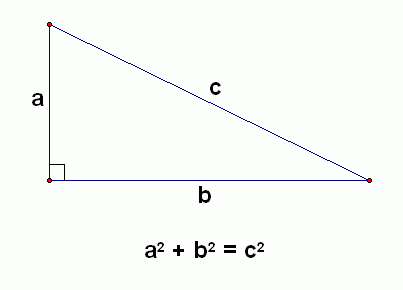
\includegraphics[scale = 0.5]{pythag.png}}

\end{enumerate}

\textbf{Pythagorean Theorem Word Problem:} A ladder leans agains the side of a house. The top of the ladder is 12ft from the ground. The bottom of the ladder is 5ft from the house. Find the length of the ladder and round to the nearest tenth.

\vspace{6cm}

\section{Factoring Polynomials (R.5)}

\textbf{Factoring} an expression means to rewrite the expression as an equivalent product. There are 5 methods of factoring at our disposal and of the special factoring types we have 4 different forms:

\begin{enumerate}

\item Factoring using the Greatest Common Factor (GCF)

\begin{itemize}

\item The GCF is the largest factor common to all terms in a polynomial

\end{itemize}

\item Factoring Common Binomial Factors
\item Factoring by Grouping
\item Factoring Quadratic Polynomials
\item Factoring Special Types

\begin{enumerate}

\item Factoring Difference of Two Squares
\newline

\centerline{Rule: $x^2 - y^2 = (x-y)(x+y)$}

\item Factoring Perfect Square Trinomials
\newline

\centerline{Rule 1: $x^2 + 2xy + y^2 = (x+y)^2$}

\centerline{Rule 2: $x^2 - 2xy + y^2 = (x-y)^2$}

\item Factoring Sum/Difference of Two Perfect Cubes
\newline

\centerline{Rule 1: $x^3 + y^3 = (x+y)(x^2 - xy + y^2)$}

\centerline{Rule 2: $x^3 - y^3 = (x-y)(x^2 + xy + y^2)$}

\item Factoring Quadratic-like Polynomials using u-Substitution

\end{enumerate}

\end{enumerate}

%\section{Rational Expressions (R.6)}
%
%Often times in Mathematics we encounter expressions called \textbf{Rational Expressions}. A rational expression is one that can be written as the quotient of two polynomials. In this section we learn how to do the following:
%
%\begin{enumerate}
%
%\item Simplify rational expressions
%
%\begin{itemize}
%
%\item To \textbf{simplify} a rational expression means to cancel any common factors between the numerator and denominator
%
%\end{itemize}
%
%\item Multiply/Divide rational expressions
%\item Add/Subtract rational expressions
%\item Simplify compound fractions
%\begin{itemize}
%
%\item A \textbf{compound fraction} is a rational  expression whose numerator or denominator contains a fraction
%
%\end{itemize}
%
%
%\end{enumerate}













\end{document}